\documentclass[border=4pt,12pt]{standalone}
% House style for redrawn exam diagrams (diagram-v4: 0.4pt lines, filled -latex arrows, fine dashes; stipple and hatching drawn as real dots/lines (no PDF/SVG patterns, so they render in every browser and at any scale); transparent background). Every figure \input's this.
\usepackage{amsmath,amssymb}
\usepackage{txfonts}
\usepackage{pdfrender,xcolor}
% \halo{text}: label on shading. The shading stops just around each letter's outline (a thin knock-out that follows the
% glyphs, like the papers' typesetting), never a box. Owner: "I don't want a box around the text".
\newcommand{\halo}[1]{\leavevmode\rlap{\pdfrender{TextRenderingMode=2,LineWidth=2.2pt,LineJoinStyle=1,StrokeColor=white,FillColor=white}#1}#1}
\usepackage{tikz,pgfplots}
\pgfplotsset{compat=1.18}
\usetikzlibrary{arrows.meta,calc,angles,quotes,patterns,patterns.meta,intersections,positioning,decorations.markings,shapes.geometric}
% Stipple and hatching are drawn as actual dots / lines clipped to the region (path picture), NOT as pattern fills:
% SVG <pattern> fills vanish or blur when browsers scale the image, so the owner could not see the shading.
% Each dot is a 0.72pt square (keeps SVGs small; reads as a dot at print size). Dots sit on one global staggered grid, so neighbouring regions line up.
\makeatletter
\newdimen\ex@x \newdimen\ex@y \newdimen\ex@xa \newdimen\ex@ya \newdimen\ex@xb \newdimen\ex@yb \newcount\ex@row
\def\exam@stipplecolor{black!75}\def\exam@dotr{0.42pt}\def\exam@dotgap{2.5}
\def\ex@rowdots{\ifdim\ex@x<\ex@xb \pgfpathrectangle{\pgfqpoint{\dimexpr\ex@x-0.36pt\relax}{\dimexpr\ex@y-0.36pt\relax}}{\pgfqpoint{0.72pt}{0.72pt}}\advance\ex@x by \exam@dotgap pt\relax\expandafter\ex@rowdots\fi}
\def\exam@stipple{%
  \pgftransformreset% dots are sized in real points even inside scaled pictures
  \pgfpointanchor{path picture bounding box}{south west}\ex@xa=\pgf@x \ex@ya=\pgf@y
  \pgfpointanchor{path picture bounding box}{north east}\ex@xb=\pgf@x \ex@yb=\pgf@y
  \pgfsetfillcolor{\exam@stipplecolor}\pgfmathsetmacro\ex@h{\exam@dotgap/2}%
  \pgfmathtruncatemacro\ex@r{floor(\ex@ya/\ex@h)-1}\ex@row=\ex@r\relax
  \ex@y=\ex@r\dimexpr\ex@h pt\relax
  \loop\ifdim\ex@y<\ex@yb
    \pgfmathtruncatemacro\ex@c{floor(\ex@xa/\exam@dotgap)-1}\ex@x=\ex@c\dimexpr\exam@dotgap pt\relax
    \ifodd\ex@row \advance\ex@x by \ex@h pt\fi
    \ex@rowdots
    \advance\ex@y by \ex@h pt \advance\ex@row by 1
    \ifnum\numexpr\ex@row-(\ex@row/4)*4\relax=0 \pgfusepath{fill}\fi% flush every 4 rows: bounded TeX memory, few clip copies in the SVG
  \repeat\pgfusepath{fill}}
\newdimen\ex@d
\def\exam@hatch#1{% #1 = 1 for /, -1 for \ ; lines 45 degrees, 3pt apart
  \pgftransformreset
  \pgfpointanchor{path picture bounding box}{south west}\ex@xa=\pgf@x \ex@ya=\pgf@y
  \pgfpointanchor{path picture bounding box}{north east}\ex@xb=\pgf@x \ex@yb=\pgf@y
  \ex@d=\dimexpr\ex@yb-\ex@ya\relax \ex@x=\dimexpr\ex@xa-\ex@d\relax
  \loop\ifdim\ex@x<\ex@xb
    \ifnum#1>0 \pgfpathmoveto{\pgfqpoint{\ex@x}{\ex@ya}}\pgfpathlineto{\pgfqpoint{\dimexpr\ex@x+\ex@d\relax}{\ex@yb}}%
    \else \pgfpathmoveto{\pgfqpoint{\ex@x}{\ex@yb}}\pgfpathlineto{\pgfqpoint{\dimexpr\ex@x+\ex@d\relax}{\ex@ya}}\fi
    \advance\ex@x by 4.24pt
  \repeat
  \pgfsetlinewidth{0.4pt}\pgfsetstrokecolor{black}\pgfusepath{stroke}}
\def\examstipple{\exam@stipple}\def\examhatch{\exam@hatch}\def\examsetstipplecolor#1{\def\exam@stipplecolor{#1}}\def\examsetdotgap#1{\def\exam@dotgap{#1}}
\makeatother
% (legacy pattern kept for old files)
% staggered stipple like the NESA papers' dotted shading
\pgfdeclarepatternformonly{exam stipple}{\pgfpointorigin}{\pgfqpoint{2.2pt}{2.2pt}}{\pgfqpoint{2.2pt}{2.2pt}}{%
  \pgfpathcircle{\pgfqpoint{0.55pt}{0.55pt}}{0.42pt}\pgfpathcircle{\pgfqpoint{1.65pt}{1.65pt}}{0.42pt}\pgfusepath{fill}}
\tikzset{
  every picture/.style={line width=0.6pt, >={Latex[length=2mm,width=1.3mm]}},
  curve/.style={line width=0.6pt},
  open arrow/.style={-{Latex[length=2mm,width=1.3mm]}},  % owner: filled -latex heads everywhere, no open chevrons
  aux/.style={dash pattern=on 2pt off 1.5pt, line width=0.6pt},
  shade/.code={\def\exA{#1}\def\exB{none}\ifx\exA\exB\else\pgfkeysalso{fill=black!18}\fi},
  shade/.default=on,
  shade dots/.style={fill=none, path picture={\examstipple}},
  stipple color/.code={\examsetstipplecolor{#1}},
  stipple gap/.code={\examsetdotgap{#1}},
  shade dense dots/.style={fill=none, stipple gap=1.6, path picture={\examstipple}},
  shade hatch/.style={fill=none, path picture={\examhatch{1}}},
  shade hatch reverse/.style={fill=none, path picture={\examhatch{-1}}},
  shade solid/.style={fill=black},
  pt/.style={circle, fill, inner sep=1.1pt},
  open pt/.style={circle, draw, fill=white, inner sep=1.1pt},
}
\pgfplotsset{
  exam axes/.style={axis lines=middle, axis line style={->}, xlabel={$x$}, ylabel={$y$},
    xlabel style={anchor=west}, ylabel style={anchor=south}, tick label style={font=\small},
    every axis plot/.append style={line width=0.6pt, black}, samples=200, clip=false,
    enlargelimits=false, axis on top},
}

\begin{document}
% option B: y=f(x+3); shared frame for options A-D: 1 unit = 37 px across, 35.5 px up (crop pixels)
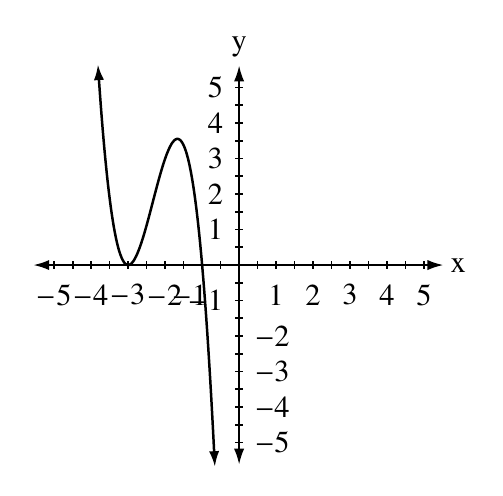
\begin{tikzpicture}[x=0.0127cm,y=-0.0127cm,every node/.style={font=\fontsize{11}{13}\selectfont}]
  \draw[<->] (24.3,250.0) -- (434.2,250.0);
  \draw[<->] (230.0,449.5) -- (230.0,50.5);
  \draw (45.0,246.3) -- (45.0,253.7); \draw (226.3,427.5) -- (233.7,427.5);
  \draw (63.5,246.3) -- (63.5,253.7); \draw (226.3,409.8) -- (233.7,409.8);
  \draw (82.0,246.3) -- (82.0,253.7); \draw (226.3,392.0) -- (233.7,392.0);
  \draw (100.5,246.3) -- (100.5,253.7); \draw (226.3,374.2) -- (233.7,374.2);
  \draw (119.0,246.3) -- (119.0,253.7); \draw (226.3,356.5) -- (233.7,356.5);
  \draw (137.5,246.3) -- (137.5,253.7); \draw (226.3,338.8) -- (233.7,338.8);
  \draw (156.0,246.3) -- (156.0,253.7); \draw (226.3,321.0) -- (233.7,321.0);
  \draw (174.5,246.3) -- (174.5,253.7); \draw (226.3,303.2) -- (233.7,303.2);
  \draw (193.0,246.3) -- (193.0,253.7); \draw (226.3,285.5) -- (233.7,285.5);
  \draw (211.5,246.3) -- (211.5,253.7); \draw (226.3,267.8) -- (233.7,267.8);
  \draw (248.5,246.3) -- (248.5,253.7); \draw (226.3,232.2) -- (233.7,232.2);
  \draw (267.0,246.3) -- (267.0,253.7); \draw (226.3,214.5) -- (233.7,214.5);
  \draw (285.5,246.3) -- (285.5,253.7); \draw (226.3,196.8) -- (233.7,196.8);
  \draw (304.0,246.3) -- (304.0,253.7); \draw (226.3,179.0) -- (233.7,179.0);
  \draw (322.5,246.3) -- (322.5,253.7); \draw (226.3,161.2) -- (233.7,161.2);
  \draw (341.0,246.3) -- (341.0,253.7); \draw (226.3,143.5) -- (233.7,143.5);
  \draw (359.5,246.3) -- (359.5,253.7); \draw (226.3,125.8) -- (233.7,125.8);
  \draw (378.0,246.3) -- (378.0,253.7); \draw (226.3,108.0) -- (233.7,108.0);
  \draw (396.5,246.3) -- (396.5,253.7); \draw (226.3,90.2) -- (233.7,90.2);
  \draw (415.0,246.3) -- (415.0,253.7); \draw (226.3,72.5) -- (233.7,72.5);
  \node at (45.0,279.9) {$-5$};
  \node[anchor=west] at (235.9,427.5) {$-5$};
  \node at (82.0,279.9) {$-4$};
  \node[anchor=west] at (235.9,392.0) {$-4$};
  \node at (119.0,279.9) {$-3$};
  \node[anchor=west] at (235.9,356.5) {$-3$};
  \node at (156.0,279.9) {$-2$};
  \node[anchor=west] at (235.9,321.0) {$-2$};
  \node at (181.0,279.9) {$-1$};
  \node[anchor=east] at (224.1,285.5) {$-1$};
  \node at (267.0,279.9) {$1$};
  \node[anchor=east] at (224.1,214.5) {$1$};
  \node at (304.0,279.9) {$2$};
  \node[anchor=east] at (224.1,179.0) {$2$};
  \node at (341.0,279.9) {$3$};
  \node[anchor=east] at (224.1,143.5) {$3$};
  \node at (378.0,279.9) {$4$};
  \node[anchor=east] at (224.1,108.0) {$4$};
  \node at (415.0,279.9) {$5$};
  \node[anchor=east] at (224.1,72.5) {$5$};
  \node at (449.1,251.0) {x};
  \node at (230.0,32.0) {y};
  \draw[<->,line width=0.9pt] plot[domain=-0.818:2.345,smooth,samples=90] ({230.00+37.000*(\x-3)},{250.00-35.500*(6*(\x)^2-3*(\x)^3)});
\end{tikzpicture}
\end{document}
